\PassOptionsToPackage{unicode=true}{hyperref} % options for packages loaded elsewhere
\PassOptionsToPackage{hyphens}{url}
%
\documentclass[
  spanish,
  ignorenonframetext,
]{beamer}
\usepackage{pgfpages}
\setbeamertemplate{caption}[numbered]
\setbeamertemplate{caption label separator}{: }
\setbeamercolor{caption name}{fg=normal text.fg}
\beamertemplatenavigationsymbolsempty
% Prevent slide breaks in the middle of a paragraph:
\widowpenalties 1 10000
\raggedbottom
\setbeamertemplate{part page}{
  \centering
  \begin{beamercolorbox}[sep=16pt,center]{part title}
    \usebeamerfont{part title}\insertpart\par
  \end{beamercolorbox}
}
\setbeamertemplate{section page}{
  \centering
  \begin{beamercolorbox}[sep=12pt,center]{part title}
    \usebeamerfont{section title}\insertsection\par
  \end{beamercolorbox}
}
\setbeamertemplate{subsection page}{
  \centering
  \begin{beamercolorbox}[sep=8pt,center]{part title}
    \usebeamerfont{subsection title}\insertsubsection\par
  \end{beamercolorbox}
}
\AtBeginPart{
  \frame{\partpage}
}
\AtBeginSection{
  \ifbibliography
  \else
    \frame{\sectionpage}
  \fi
}
\AtBeginSubsection{
  \frame{\subsectionpage}
}
\usepackage{lmodern}
\usepackage{amssymb,amsmath}
\usepackage{ifxetex,ifluatex}
\ifnum 0\ifxetex 1\fi\ifluatex 1\fi=0 % if pdftex
  \usepackage[T1]{fontenc}
  \usepackage[utf8]{inputenc}
  \usepackage{textcomp} % provides euro and other symbols
\else % if luatex or xelatex
  \usepackage{unicode-math}
  \defaultfontfeatures{Scale=MatchLowercase}
  \defaultfontfeatures[\rmfamily]{Ligatures=TeX,Scale=1}
\fi
\usetheme[]{Boadilla}
\usecolortheme{beaver}
% use upquote if available, for straight quotes in verbatim environments
\IfFileExists{upquote.sty}{\usepackage{upquote}}{}
\IfFileExists{microtype.sty}{% use microtype if available
  \usepackage[]{microtype}
  \UseMicrotypeSet[protrusion]{basicmath} % disable protrusion for tt fonts
}{}
\makeatletter
\@ifundefined{KOMAClassName}{% if non-KOMA class
  \IfFileExists{parskip.sty}{%
    \usepackage{parskip}
  }{% else
    \setlength{\parindent}{0pt}
    \setlength{\parskip}{6pt plus 2pt minus 1pt}}
}{% if KOMA class
  \KOMAoptions{parskip=half}}
\makeatother
\usepackage{xcolor}
\IfFileExists{xurl.sty}{\usepackage{xurl}}{} % add URL line breaks if available
\IfFileExists{bookmark.sty}{\usepackage{bookmark}}{\usepackage{hyperref}}
\hypersetup{
  pdfauthor={Martín Ezequiel Langberg},
  pdfborder={0 0 0},
  breaklinks=true}
\urlstyle{same}  % don't use monospace font for urls
\newif\ifbibliography
\usepackage{longtable,booktabs}
\usepackage{caption}
% These lines are needed to make table captions work with longtable:
\makeatletter
\def\fnum@table{\tablename~\thetable}
\makeatother
\usepackage{graphicx,grffile}
\makeatletter
\def\maxwidth{\ifdim\Gin@nat@width>\linewidth\linewidth\else\Gin@nat@width\fi}
\def\maxheight{\ifdim\Gin@nat@height>\textheight\textheight\else\Gin@nat@height\fi}
\makeatother
% Scale images if necessary, so that they will not overflow the page
% margins by default, and it is still possible to overwrite the defaults
% using explicit options in \includegraphics[width, height, ...]{}
\setkeys{Gin}{width=\maxwidth,height=\maxheight,keepaspectratio}
\setlength{\emergencystretch}{3em}  % prevent overfull lines
\providecommand{\tightlist}{%
  \setlength{\itemsep}{0pt}\setlength{\parskip}{0pt}}
\setcounter{secnumdepth}{-2}

% set default figure placement to htbp
\makeatletter
\def\fps@figure{htbp}
\makeatother

\usepackage{caption}
\captionsetup[figure]{labelformat=empty}
\ifnum 0\ifxetex 1\fi=0 % if pdftex or luatex
  \usepackage[shorthands=off,main=spanish]{babel}
\else % if xetex
  % load polyglossia as late as possible as it *could* call bidi if RTL lang (e.g. Hebrew or Arabic)
  \usepackage{polyglossia}
  \setmainlanguage[]{spanish}
\fi

\title{Predicción de patogenicidad en SNPs}
\author{Martín Ezequiel Langberg}
\date{}

\begin{document}
\frame{\titlepage}

\begin{frame}{Introducción: ¿Qué son los SNPs?}
\protect\hypertarget{introducciuxf3n-quuxe9-son-los-snps}{}

\begin{figure}
\centering
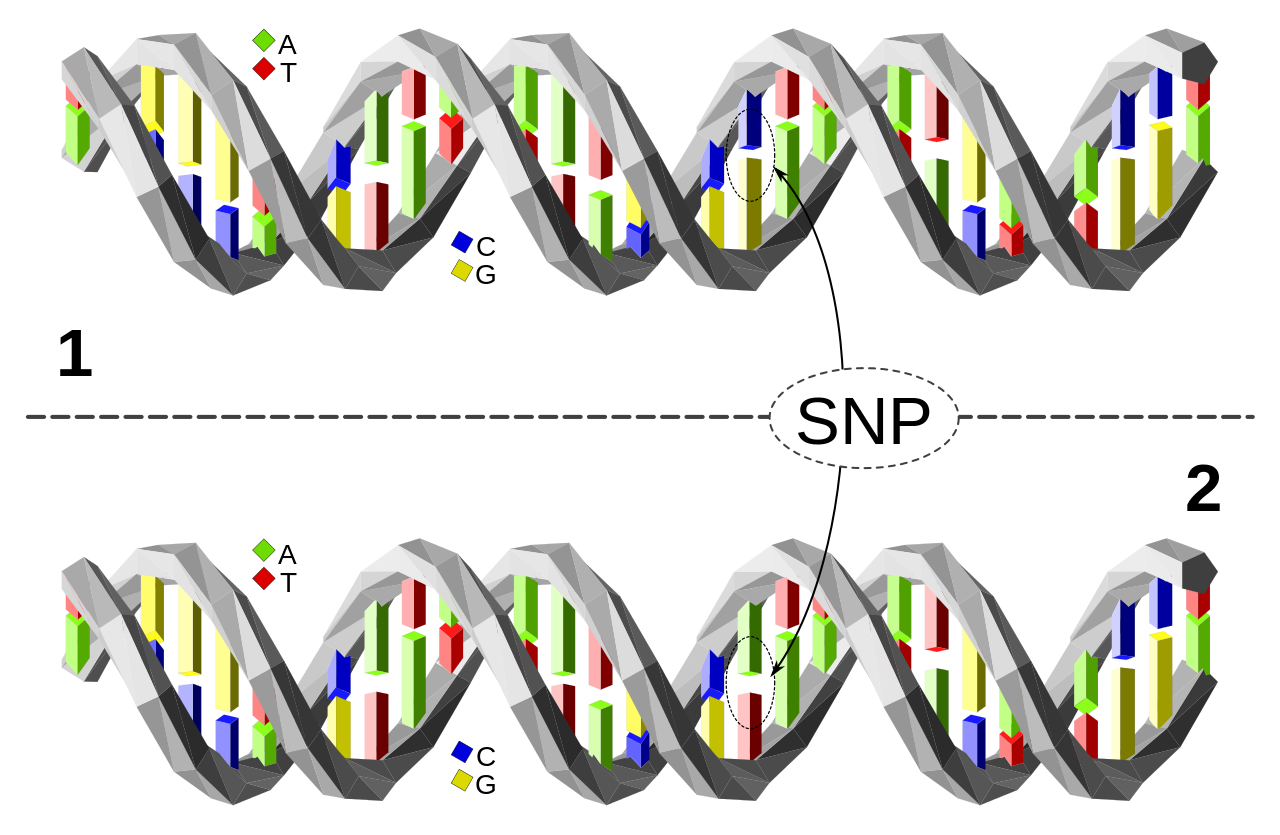
\includegraphics[width=3.64583in,height=\textheight]{Dna-SNP.svg.png}
\caption{Single Nucleotide Polymorphism (SNP)}
\end{figure}

\end{frame}

\begin{frame}{Introducción: Del ADN a las proteínas}
\protect\hypertarget{introducciuxf3n-del-adn-a-las-proteuxednas}{}

\begin{figure}
\centering
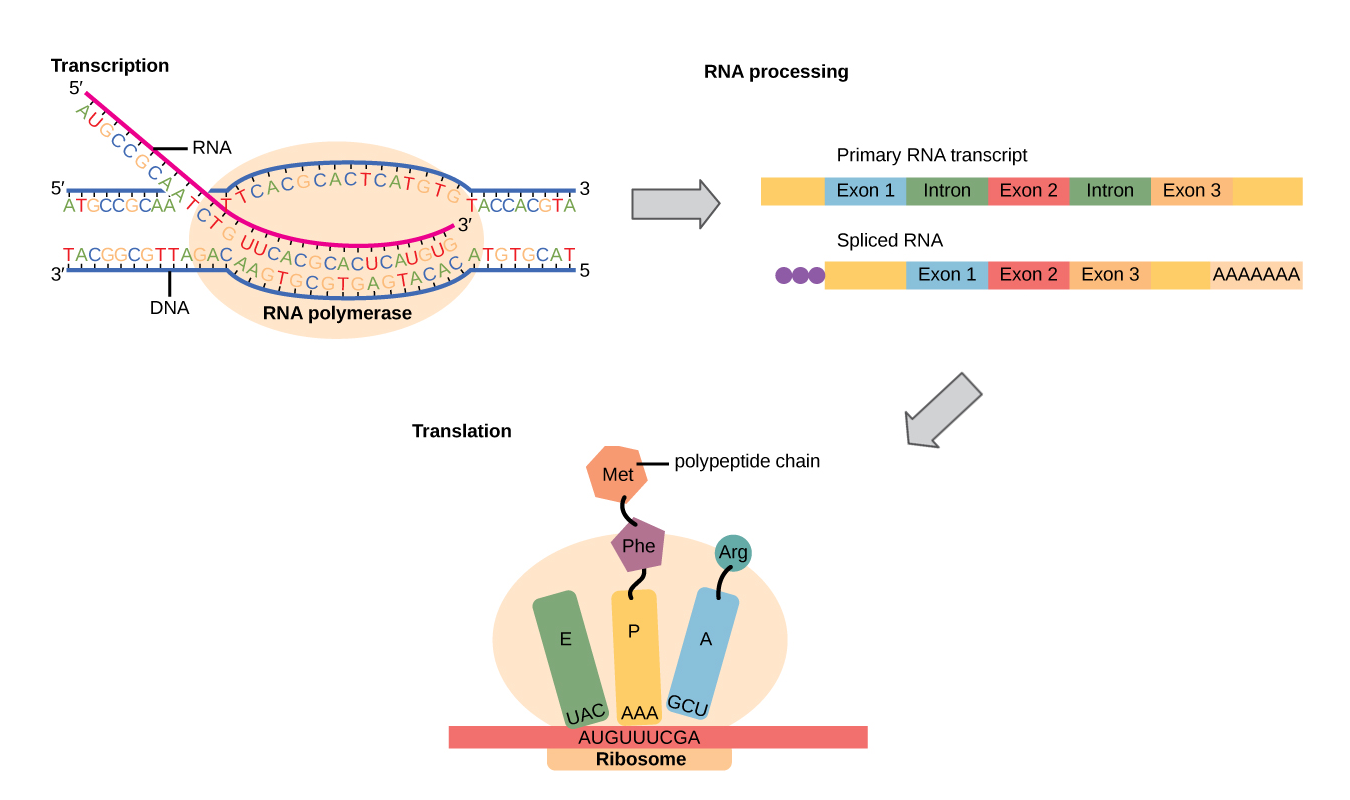
\includegraphics[width=4.6875in,height=\textheight]{dogma.png}
\caption{Dogma central de la biología}
\end{figure}

\end{frame}

\begin{frame}{¿Cómo se expresan los SNPs en el organismo?}
\protect\hypertarget{cuxf3mo-se-expresan-los-snps-en-el-organismo}{}

\begin{figure}
\centering
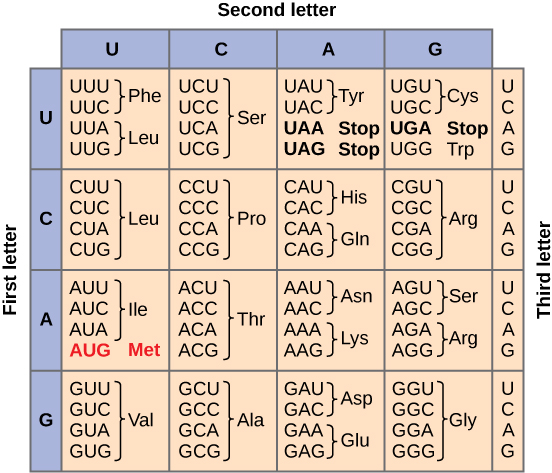
\includegraphics[width=2.60417in,height=\textheight]{tableCodon.jpg}
\caption{Tabla de codones de ARN}
\end{figure}

\end{frame}

\begin{frame}{Introducción: Tipos de SNPs}
\protect\hypertarget{introducciuxf3n-tipos-de-snps}{}

\begin{block}{Sustitución sinónima o \textit{silent}}

El cambio en el nucleótido no modifica el aminoácido

\end{block}

\begin{figure}
\centering
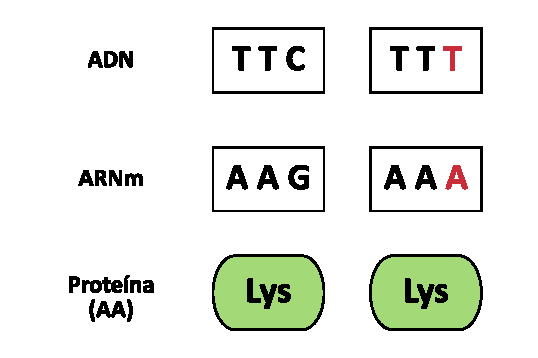
\includegraphics[width=2.60417in,height=\textheight]{silent_mutation.pdf}
\caption{Sustitución \textit{silent}}
\end{figure}

\end{frame}

\begin{frame}{Introducción: Tipos de SNPs}
\protect\hypertarget{introducciuxf3n-tipos-de-snps-1}{}

\begin{block}{Sustituciones no sinónimas}

Nonsense: Generan un codón de terminación o \textit{stop}

\end{block}

\begin{figure}
\centering
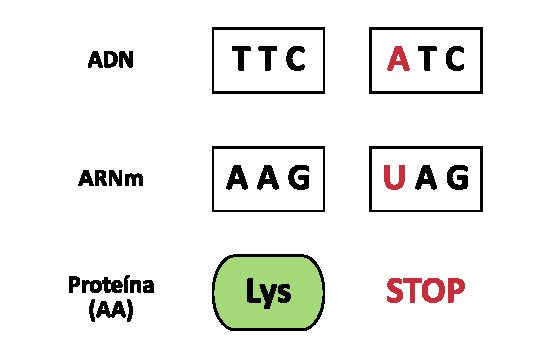
\includegraphics[width=2.60417in,height=\textheight]{nonsense_mutation.pdf}
\caption{Sustitución \textit{nonsense}}
\end{figure}

\end{frame}

\begin{frame}{Introducción: Tipos de SNPs}
\protect\hypertarget{introducciuxf3n-tipos-de-snps-2}{}

\begin{block}{Sustituciones no sinónimas}

Missense: Generan un cambio de aminoácido en la proteína

\end{block}

\begin{figure}
\centering
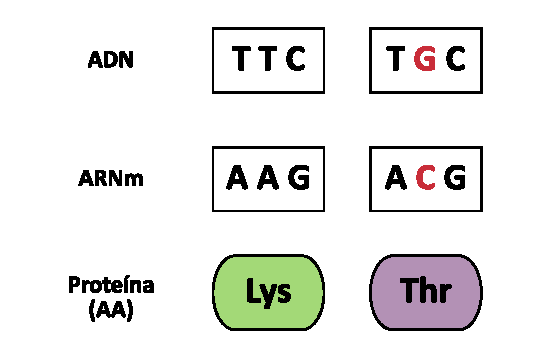
\includegraphics[width=2.60417in,height=\textheight]{missense_mutation.pdf}
\caption{Sustitución \textit{missense}}
\end{figure}

\end{frame}

\begin{frame}{Foco de estudio: Variantes \textit{missense}}
\protect\hypertarget{foco-de-estudio-variantes}{}

\begin{block}{Sustitución sinónima o \textit{silent}}

\begin{itemize}
\tightlist
\item
  El cambio en el nucleótido no modifica el aminoácido
\end{itemize}

\end{block}

\begin{block}{Sustituciones no sinónimas}

\begin{itemize}
\tightlist
\item
  Nonsense: Generan un codón de terminación o \textit{stop}
\item
  Missense: Generan un cambio de aminoácido en la proteína
\end{itemize}

\end{block}

\begin{figure}
\centering
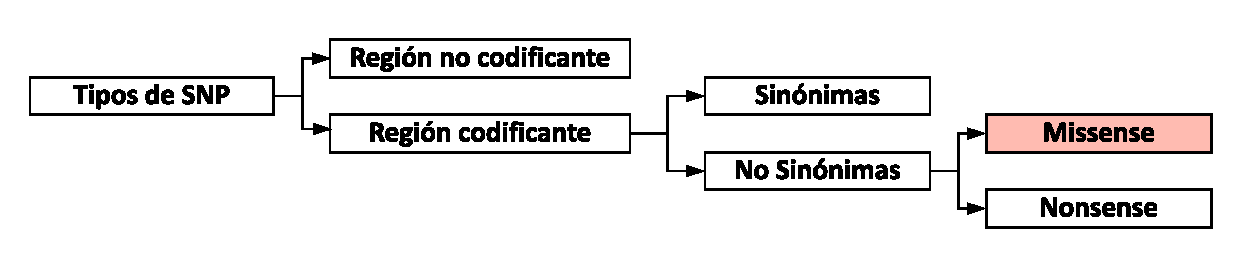
\includegraphics{snp_types.pdf}
\caption{Tipos de SNPs}
\end{figure}

\end{frame}

\begin{frame}{Problema biológico: detectar la patogenicidad de SNPs}
\protect\hypertarget{problema-bioluxf3gico-detectar-la-patogenicidad-de-snps}{}

\begin{itemize}
\item
  La mayoría de las mutaciones no sinónimas son raras (AF \textless{}
  .05\%)
\item
  Los estudios realizados con secuenciación tienen baja significación
  estadística
\item
  Existen bases de datos biológicas que registran patogenicidad de
  mutaciones: Clinvar, Humsavar y otras

  \begin{longtable}[]{@{}llll@{}}
  \toprule
  Main gene name & AA change & Type of variant & dbSNP\tabularnewline
  \midrule
  \endhead
  A4GALT & p.Pro251Leu & Polymorphism & rs28940571\tabularnewline
  A4GALT & p.Gln163Arg & Polymorphism & rs28915383\tabularnewline
  A4GNT & p.Ala218Asp & Polymorphism & rs2246945\tabularnewline
  AAAS & p.His160Arg & Disease & -\tabularnewline
  AAAS & p.Ser263Pro & Disease & rs121918550\tabularnewline
  \bottomrule
  \end{longtable}

  \center{Selección de columnas de tabla Humsavar (extracto)}
\end{itemize}

\end{frame}

\begin{frame}{Enfoque computacional: un problema de clasificación}
\protect\hypertarget{enfoque-computacional-un-problema-de-clasificaciuxf3n}{}

\begin{itemize}
\item
  \textbf{Objetivo: Predecir patogenicidad de SNPs \textit{missense}
  humanos}
\item
  Trabajos previos:

  \begin{itemize}
  \tightlist
  \item
    VEST (Carter et al., 2013)\\
  \item
    FATHMM-MKL (Shihab et al., 2015)
  \item
    REVEL (Ioannidis et al., 2016)
  \end{itemize}
\item
  Aprendizaje automático supervisado
\item
  Dimensiones estructurales, físico-químicas de las proteínas, genómicas
\item
  Análisis de importancia de las variables
\end{itemize}

\end{frame}

\begin{frame}{}
\protect\hypertarget{section}{}

\begin{center}
\Huge ¿Qué tan difícil es este problema?
\end{center}

\end{frame}

\begin{frame}{Primer modelo: Propiedades estructurales usando VarQ}
\protect\hypertarget{primer-modelo-propiedades-estructurales-usando-varq}{}

\begin{figure}
\centering
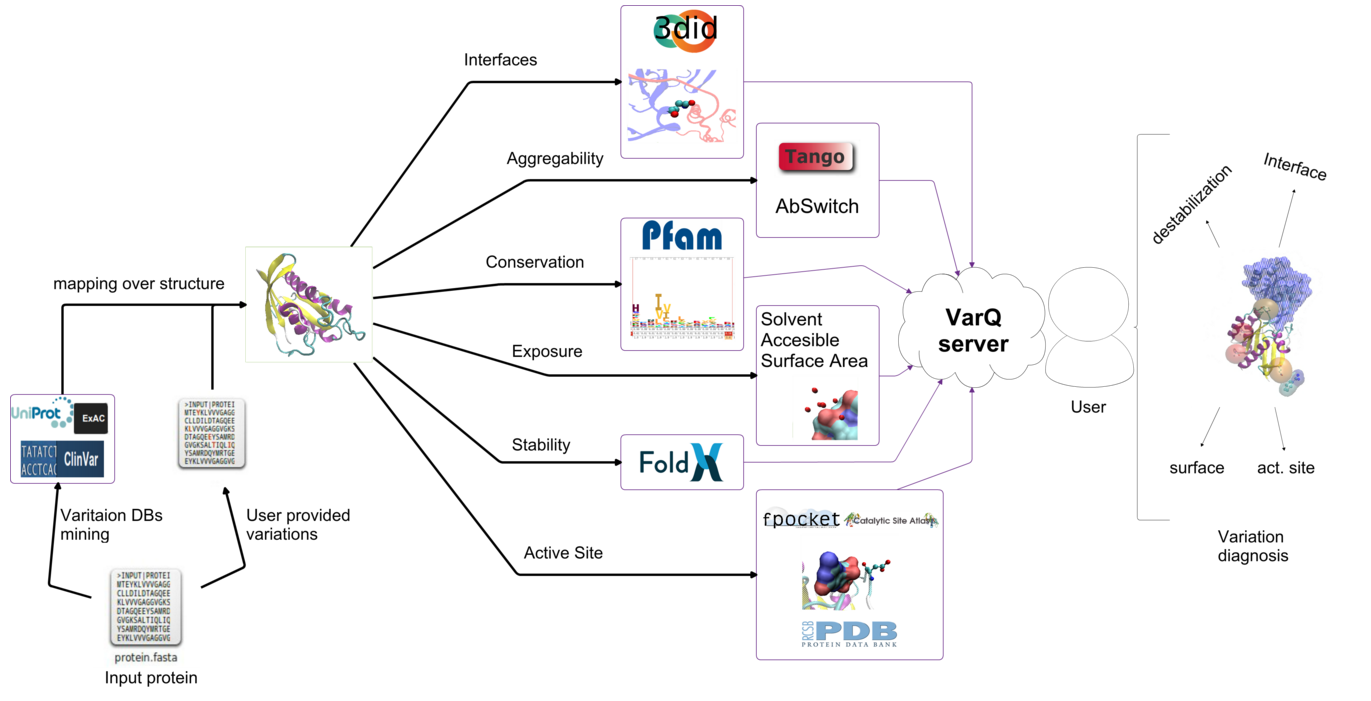
\includegraphics[width=2.60417in,height=\textheight]{varQ_Pipeline.png}
\caption{Pipeline de extracción de datos de VarQ}
\end{figure}

\begin{block}{Features extraídos (cobertura)}

\begin{columns}[T]
\begin{column}{0.48\textwidth}
\begin{itemize}
\tightlist
\item
  Variación de la energía
\item
  SASA
\item
  Porcentaje de SASA
\item
  B-Factor
\item
  Switchbility
\end{itemize}
\end{column}

\begin{column}{0.48\textwidth}
\begin{itemize}
\tightlist
\item
  Aggregability
\item
  Conservación
\item
  Interfaz 3DID
\item
  Interfaz PDB
\item
  \textbf{Active Site}
\end{itemize}
\end{column}
\end{columns}

\end{block}

\end{frame}

\begin{frame}{Filtrado de variantes del dataset VarQ}
\protect\hypertarget{filtrado-de-variantes-del-dataset-varq}{}

\begin{itemize}
\tightlist
\item
  Removimos variantes sin un status confirmado (\textit{risk factor},
  \textit{likely benign}, \textit{uncertain significance})
\item
  Priorizamos con el reporte de Humsavar (Pathogenic, Disease)
\item
  Aproximadamente 7,500 variantes: 72\% patogénicas, 28\% benignas
\end{itemize}

\begin{figure}
\centering
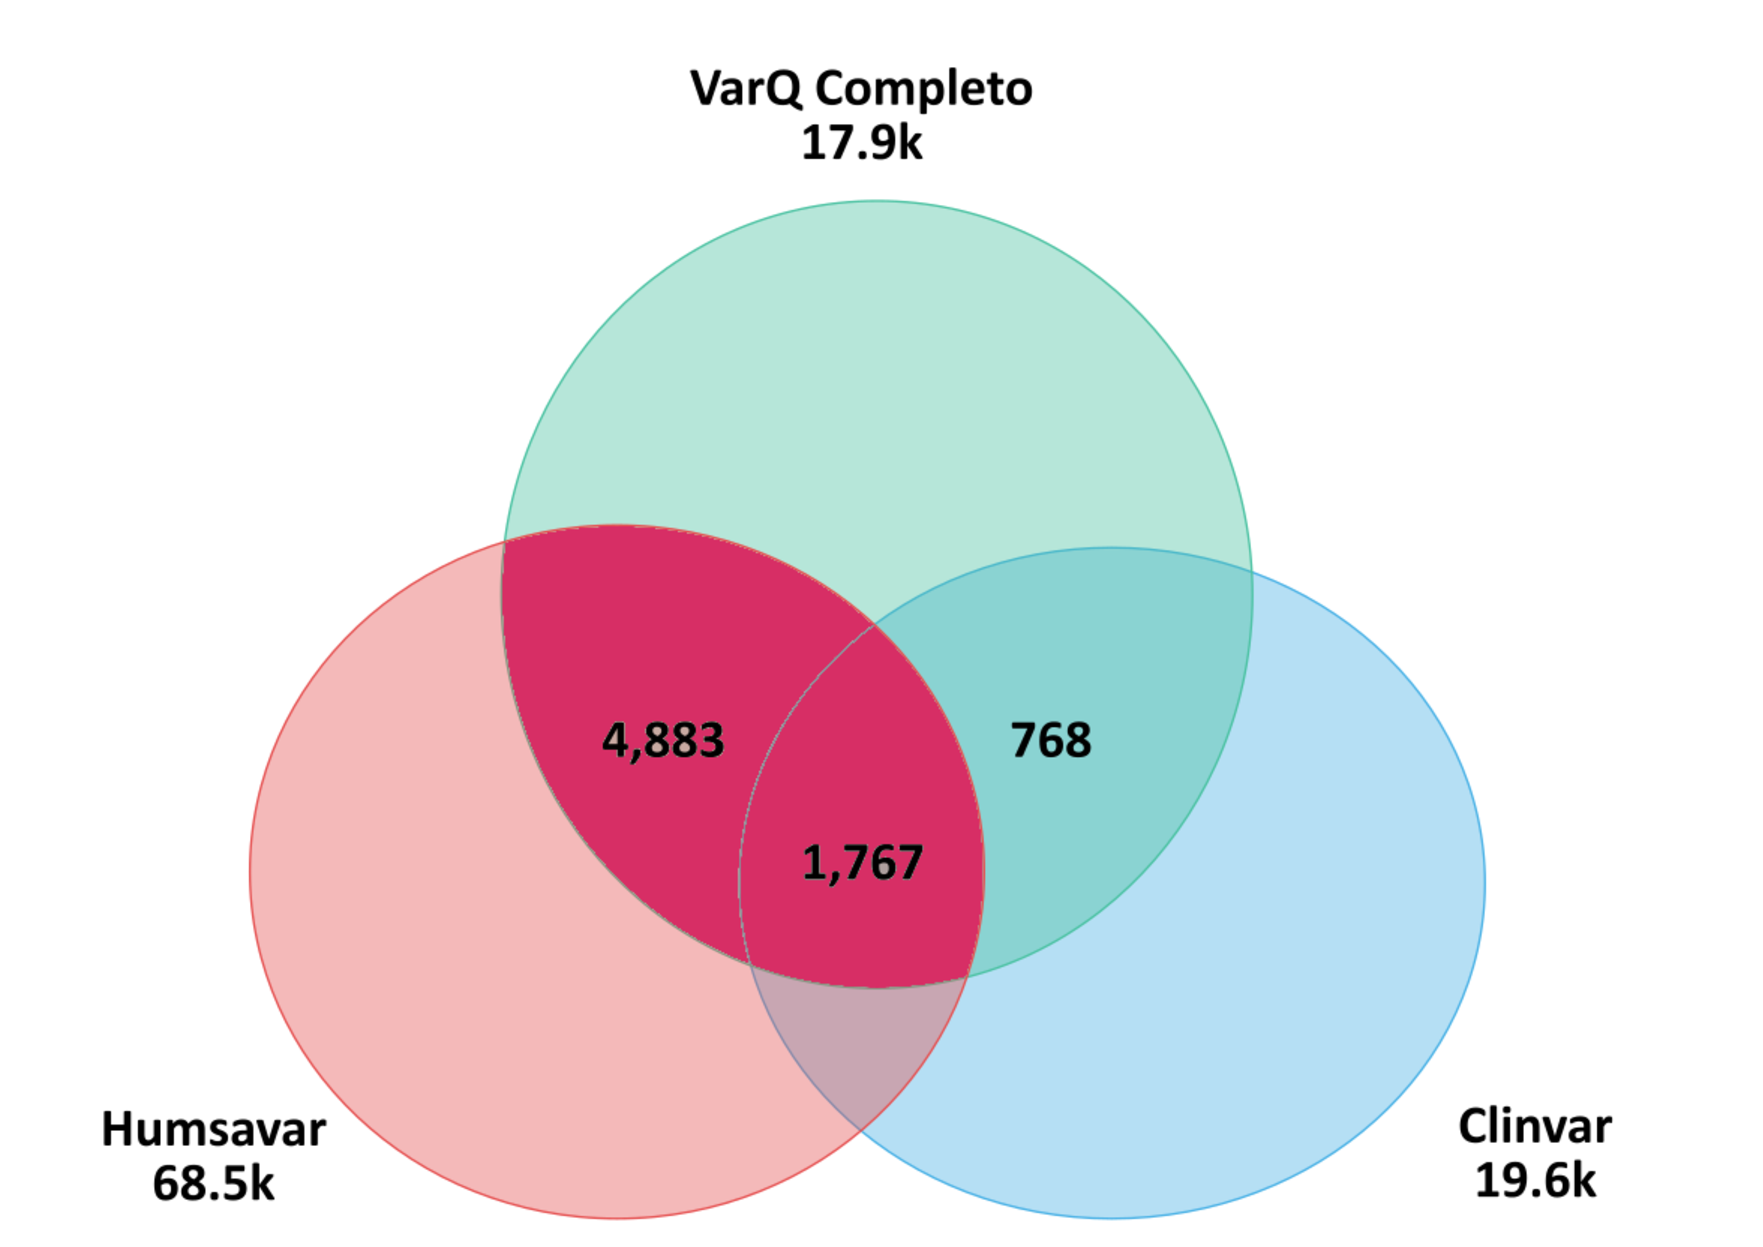
\includegraphics[width=2.08333in,height=\textheight]{interseccion_varq.pdf}
\caption{Intersección del dataset VarQ usando Humsavar y Clinvar}
\end{figure}

\end{frame}

\begin{frame}{Generación de modelos de aprendizaje automático}
\protect\hypertarget{generaciuxf3n-de-modelos-de-aprendizaje-automuxe1tico}{}

\begin{itemize}
\tightlist
\item
  Modelos clásicos usando \texttt{scikit-learn}

  \begin{itemize}
  \tightlist
  \item
    Support Vector Classifier (kernel radial)
  \item
    Random Forest
  \item
    Regresión logística
  \end{itemize}
\item
  Imputación de variables nulas
\item
  Búsqueda de hiperparámetros usando \textit{3-fold Cross Validation}
\end{itemize}

\end{frame}

\begin{frame}{Comparación de modelos usando VarQ: Random Forest tiene el
mejor AUC}
\protect\hypertarget{comparaciuxf3n-de-modelos-usando-varq-random-forest-tiene-el-mejor-auc}{}

\begin{longtable}[]{@{}llll@{}}
\toprule
& SVC & LR & RF\tabularnewline
\midrule
\endhead
Precisión & 0.72 & 0.75 & \textbf{0.77}\tabularnewline
Recall & \textbf{1.00} & 0.94 & 0.93\tabularnewline
AUC & 0.70 & 0.71 & \textbf{0.74}\tabularnewline
\(T_{fit}\) & 2m 39s & \textbf{1.17s} & 9.82s\tabularnewline
\(T_{pred}\) & 0.77s & \textbf{0.01s} & 0.11s\tabularnewline
\bottomrule
\end{longtable}

\end{frame}

\begin{frame}{Resultados del modelo VarQ (Random Forest): La variable
más importante es la Variación de la Energía}
\protect\hypertarget{resultados-del-modelo-varq-random-forest-la-variable-muxe1s-importante-es-la-variaciuxf3n-de-la-energuxeda}{}

\begin{columns}[T]
\begin{column}{0.48\textwidth}
\begin{figure}
\centering
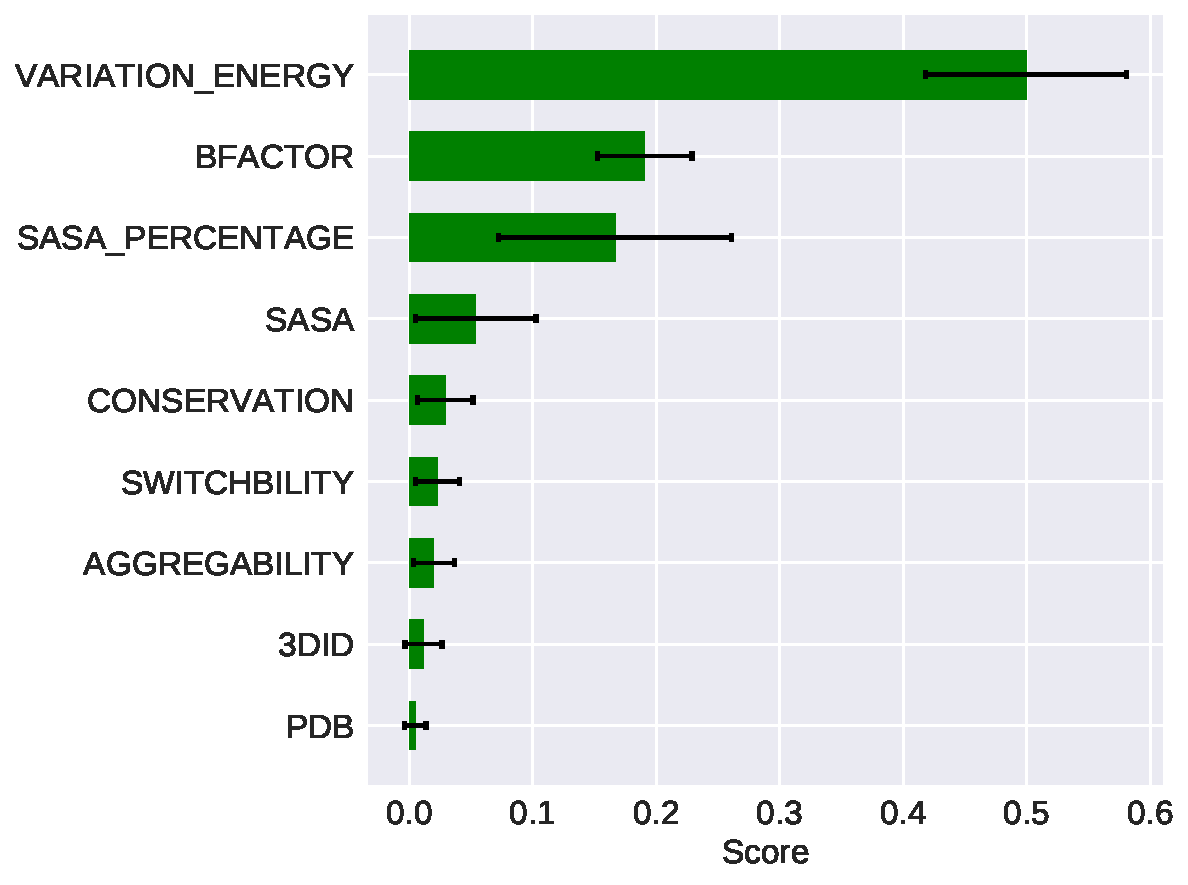
\includegraphics[width=2.60417in,height=\textheight]{importances_varq.pdf}
\caption{Importancia de variables usando método estándar de
\texttt{scikit-learn}}
\end{figure}
\end{column}

\begin{column}{0.48\textwidth}
\begin{figure}
\centering
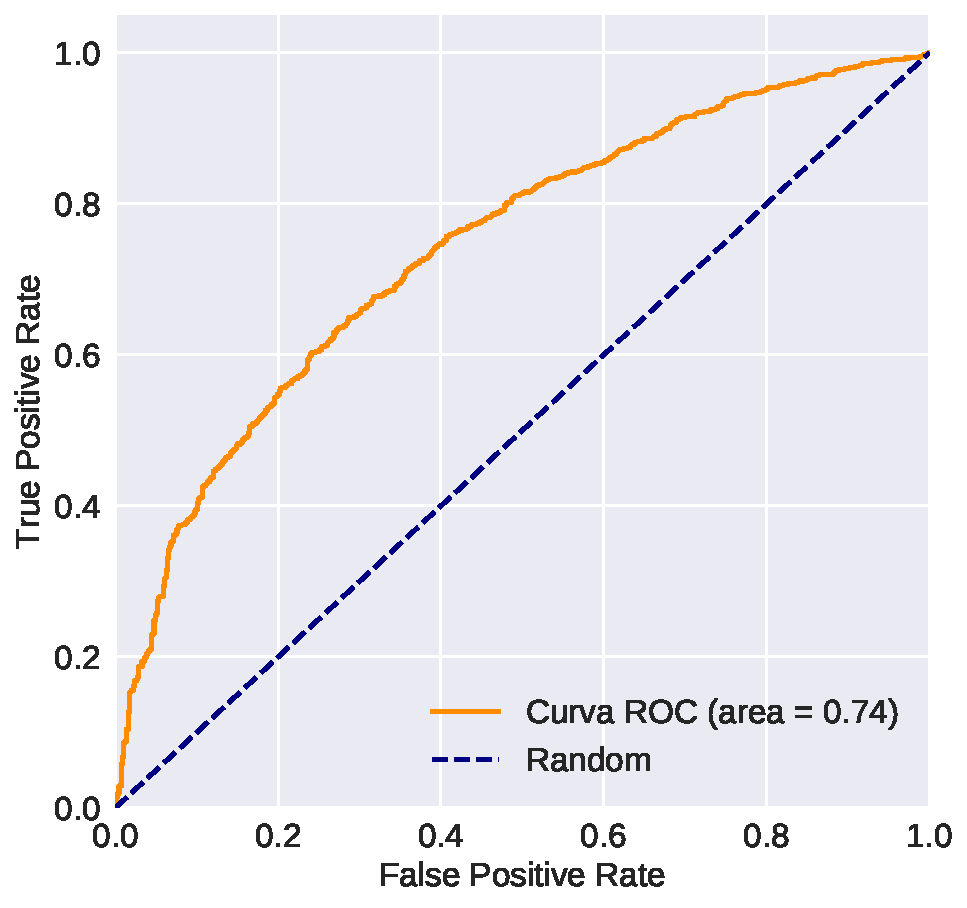
\includegraphics[width=1.77083in,height=\textheight]{auc_varq.pdf}
\caption{Curva ROC (0.74)}
\end{figure}
\end{column}
\end{columns}

\end{frame}

\begin{frame}{}
\protect\hypertarget{section-1}{}

\begin{center}
\Huge ¿Cuál es el valor predictivo de las variables fisico-químicas de la proteína?
\end{center}

\end{frame}

\begin{frame}{Modelo: Propiedades Físico-Químicas de la proteína}
\protect\hypertarget{modelo-propiedades-fuxedsico-quuxedmicas-de-la-proteuxedna}{}

\begin{itemize}
\tightlist
\item
  Uniprot: Proteoma humano completo
\item
  Nuevas fuentes de variables:

  \begin{itemize}
  \tightlist
  \item
    ProtParam (Biopython)
  \item
    SNVBox
  \end{itemize}
\item
  Usando únicamente la tabla Humsavar:

  \begin{itemize}
  \tightlist
  \item
    Más de 68 mil variantes (aprox. x10 Varq!)
  \item
    Status aportado por Humsavar
  \end{itemize}
\end{itemize}

\begin{figure}
\centering
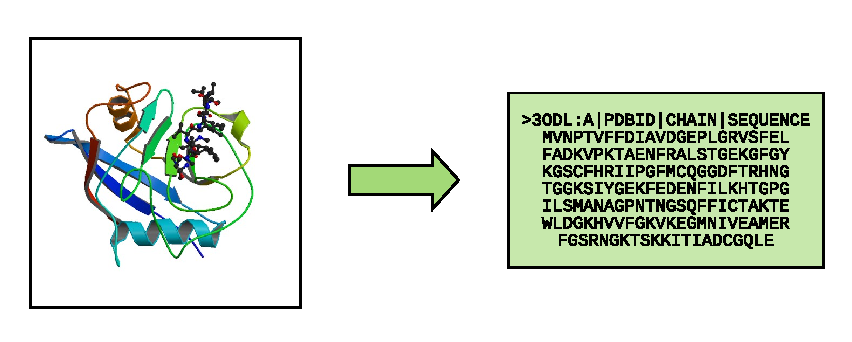
\includegraphics[width=3.64583in,height=\textheight]{fasta.pdf}
\caption{Extracción de secuencia proteica (ciclofilina) en formato FASTA
usando Uniprot}
\end{figure}

\end{frame}

\begin{frame}{Generación de nuevas variables usando ProtParam}
\protect\hypertarget{generaciuxf3n-de-nuevas-variables-usando-protparam}{}

\begin{block}{Parámetros calculados}

\begin{itemize}
\tightlist
\item
  Punto isoeléctrico
\item
  Aromaticidad
\item
  Índice de inestabilidad
\item
  Flexibilidad
\item
  Promedio de hidrofobicidad
\end{itemize}

\end{block}

\begin{block}{Cambio en la variante}

\begin{itemize}
\tightlist
\item
  Diferencia
\item
  Log-ratio
\end{itemize}

\end{block}

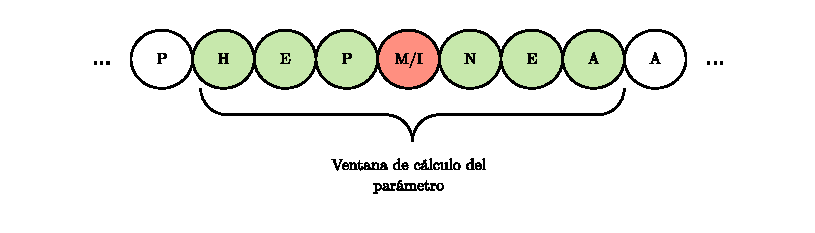
\includegraphics[width=4.42708in,height=\textheight]{protparam.pdf}

\end{frame}

\begin{frame}{Variables físico-químicas extraídas de SNVBox}
\protect\hypertarget{variables-fuxedsico-quuxedmicas-extrauxeddas-de-snvbox}{}

\begin{block}{Variables a nivel de aminoácido (considerando
sustitución)}

\begin{itemize}
\tightlist
\item
  Score BLOSUM, EX, GRANTHAM, PAM250, VB, JM
\item
  Carga
\item
  Volumen
\item
  Polaridad
\item
  Hidrofobia
\item
  Transición
\end{itemize}

\end{block}

\begin{block}{Variables a nivel de proteína (sin considerar
sustitución)}

\begin{itemize}
\tightlist
\item
  BINDING: Sitio de unión
\item
  ACTIVE\_SITE: Sitio activo
\item
  LIPID: Unión con un lípido
\item
  METAL: Unión con un metal
\item
  otras
\end{itemize}

\end{block}

\end{frame}

\begin{frame}{Las matrices fueron las más relevantes}
\protect\hypertarget{las-matrices-fueron-las-muxe1s-relevantes}{}

\begin{columns}[T]
\begin{column}{0.48\textwidth}
\begin{figure}
\centering
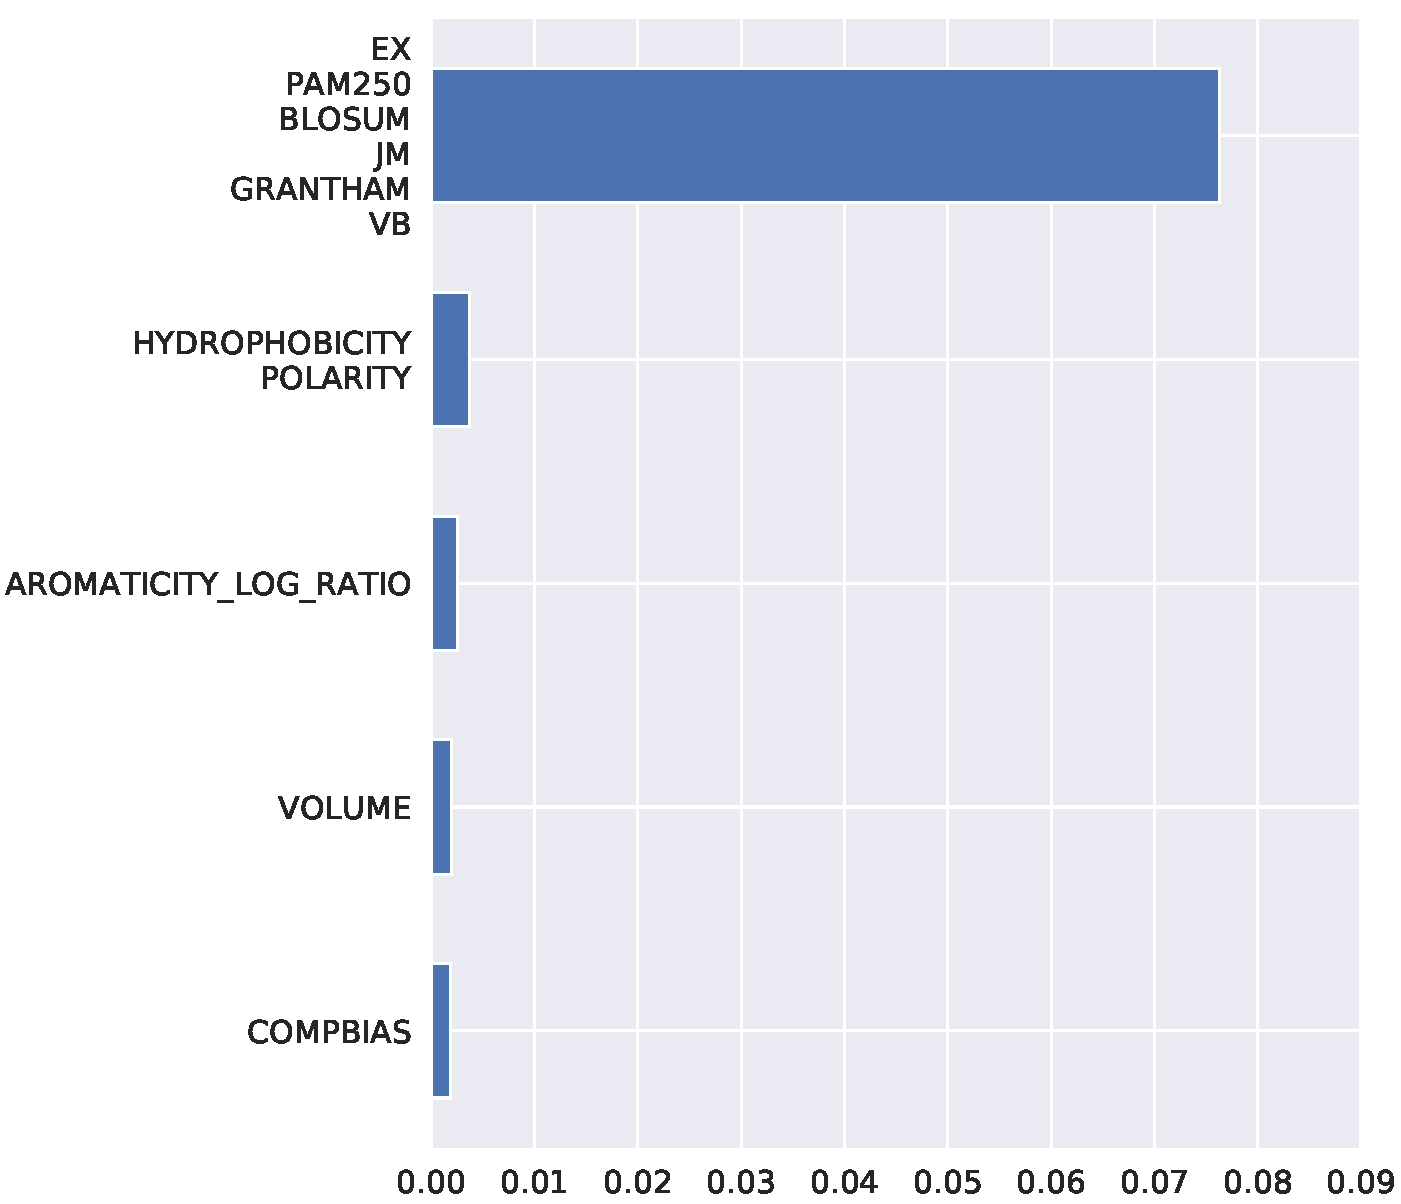
\includegraphics[width=2.39583in,height=\textheight]{structural_importance_cluster.pdf}
\caption{Importancia de variables clusterizada usando \texttt{rfpimp}}
\end{figure}
\end{column}

\begin{column}{0.48\textwidth}
\begin{figure}
\centering
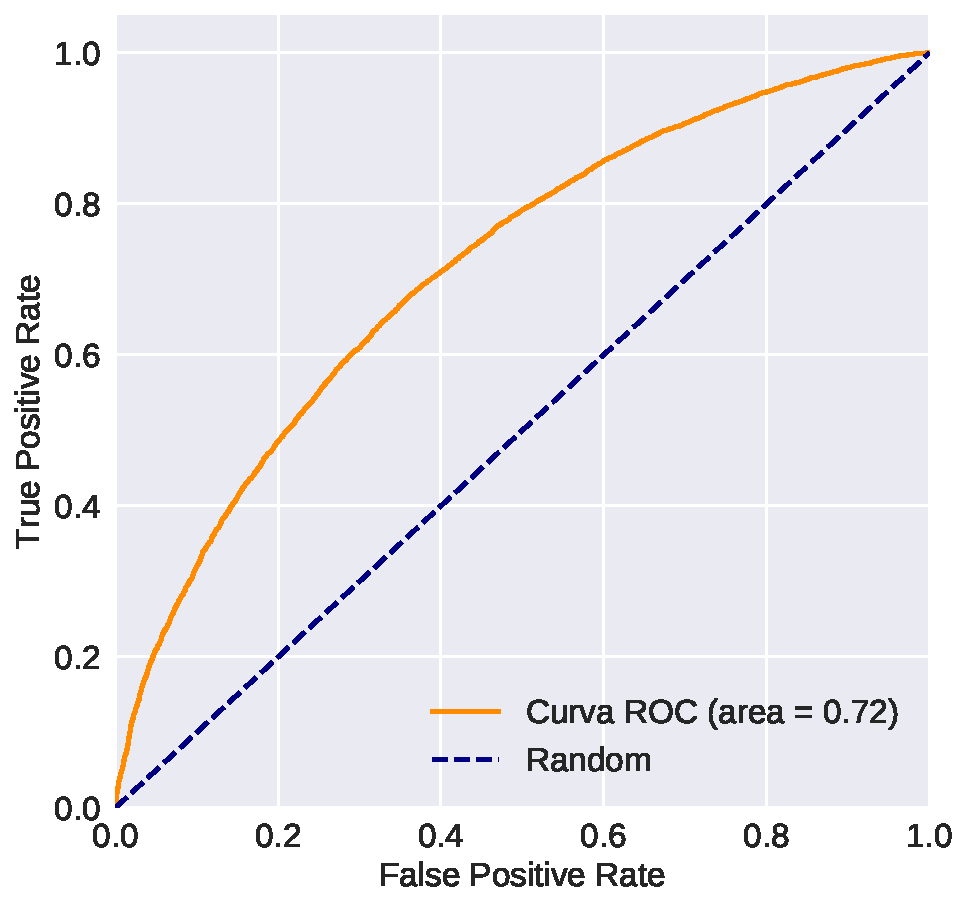
\includegraphics[width=1.92708in,height=\textheight]{auc_structural.pdf}
\caption{Curva ROC (0.72)}
\end{figure}
\end{column}
\end{columns}

\end{frame}

\begin{frame}{}
\protect\hypertarget{section-2}{}

\begin{center}
\Huge ¿Cuál es el valor predictivo de las variables genómicas?
\end{center}

\end{frame}

\begin{frame}{Modelo: Variables genómicas}
\protect\hypertarget{modelo-variables-genuxf3micas}{}

\begin{itemize}
\tightlist
\item
  Identificador rsID: aproximadamente 55,000 variantes en Humsavar

  \begin{itemize}
  \tightlist
  \item
    68\% variantes benignas
  \item
    32\% variantes patogénicas
  \end{itemize}
\item
  Fuentes de variables:

  \begin{itemize}
  \tightlist
  \item
    SNVBox
  \item
    dbSNP
  \item
    Genome Browser (UCSC)
  \end{itemize}
\end{itemize}

\begin{figure}
\centering
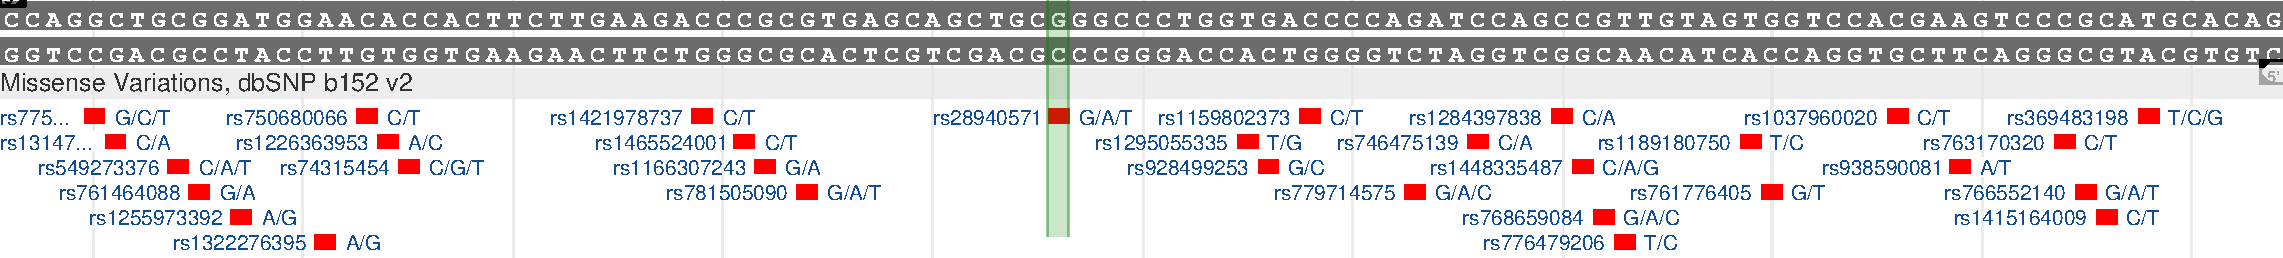
\includegraphics[width=4.6875in,height=\textheight]{variation.pdf}
\caption{Explorador de variantes de dbSNP
(\texttt{https://www.ncbi.nlm.nih.gov/snp})}
\end{figure}

\end{frame}

\begin{frame}{Variables del modelo Genómico}
\protect\hypertarget{variables-del-modelo-genuxf3mico}{}

\begin{block}{Variables de conservación genómica}

\begin{itemize}
\tightlist
\item
  PhastCons a 46 vías (vertebrados)
\item
  PhyloP a 46 vías (vertebrados)
\end{itemize}

\end{block}

\begin{block}{Variables extraídas de SNVBox}

\begin{itemize}
\tightlist
\item
  Conservación a nivel de exón
\item
  Densidad de SNPs en HapMap
\item
  Densidad de SNPs a nivel de exón
\end{itemize}

\end{block}

\begin{block}{Variables relativas a la clase funcional}

\begin{itemize}
\tightlist
\item
  Missense
\item
  Nonsense
\item
  Intrón
\item
  y otras
\end{itemize}

\end{block}

\end{frame}

\begin{frame}{La conservación genómica es importantísima!}
\protect\hypertarget{la-conservaciuxf3n-genuxf3mica-es-importantuxedsima}{}

\begin{columns}[T]
\begin{column}{0.48\textwidth}
\begin{figure}
\centering
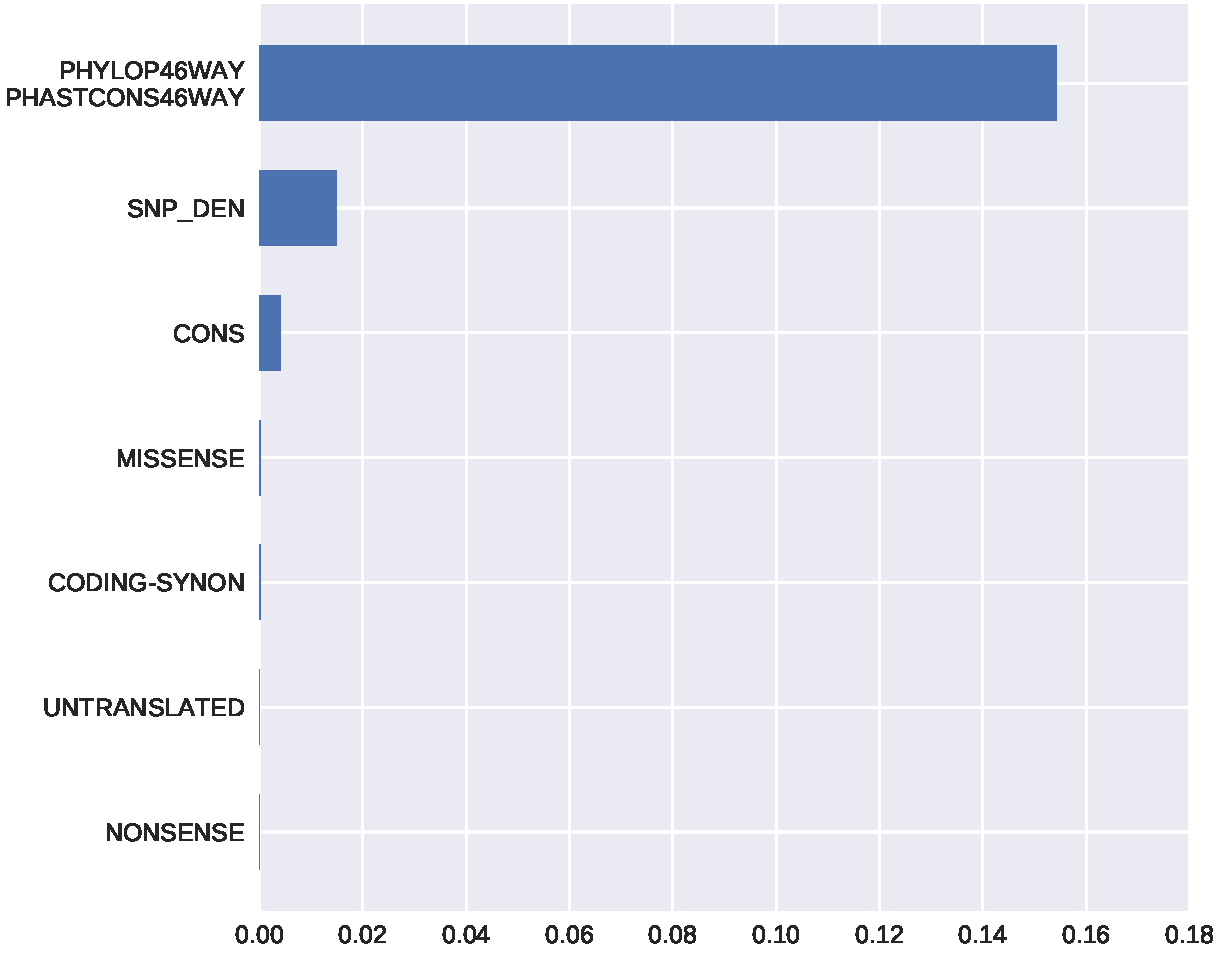
\includegraphics[width=2.44792in,height=\textheight]{genomic_importance_cluster.pdf}
\caption{Importancia de variables clusterizada usando \texttt{rfpimp}}
\end{figure}
\end{column}

\begin{column}{0.48\textwidth}
\begin{figure}
\centering
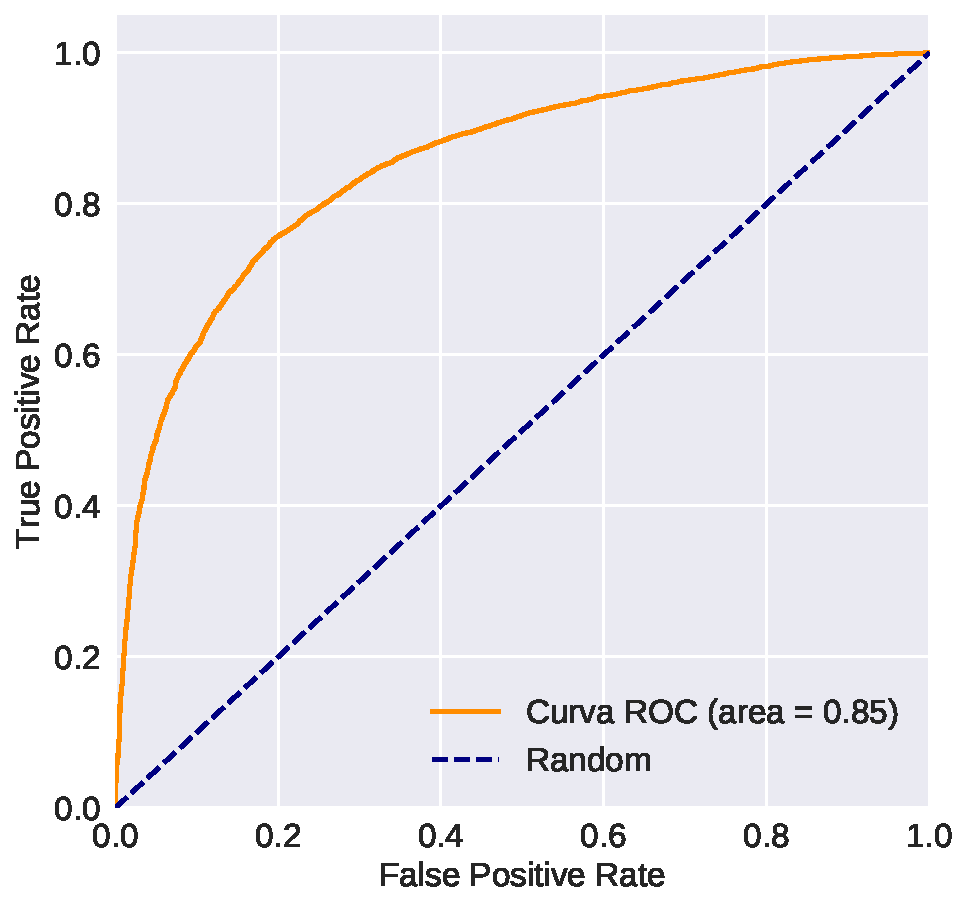
\includegraphics[width=1.82292in,height=\textheight]{auc_genomic.pdf}
\caption{Curva ROC (\textbf{0.85!})}
\end{figure}
\end{column}
\end{columns}

\end{frame}

\begin{frame}{}
\protect\hypertarget{section-3}{}

\begin{center}
\Huge Podemos mejorar el modelo genómico integrando las variables físico-químicas?
\end{center}

\end{frame}

\begin{frame}{Integrando las variables físico-químicas y genómicas}
\protect\hypertarget{integrando-las-variables-fuxedsico-quuxedmicas-y-genuxf3micas}{}

\begin{itemize}
\tightlist
\item
  Dataset Humsavar: 68 mil variantes
\item
  Cobertura variables genómicas: aprox. 80\%
\item
  Cobertura variable físico-químicas: misma que el dataset
  físico-químico
\item
  Evaluamos un nuevo método de aprendizaje automático: XGBoost
\end{itemize}

\begin{figure}
\centering
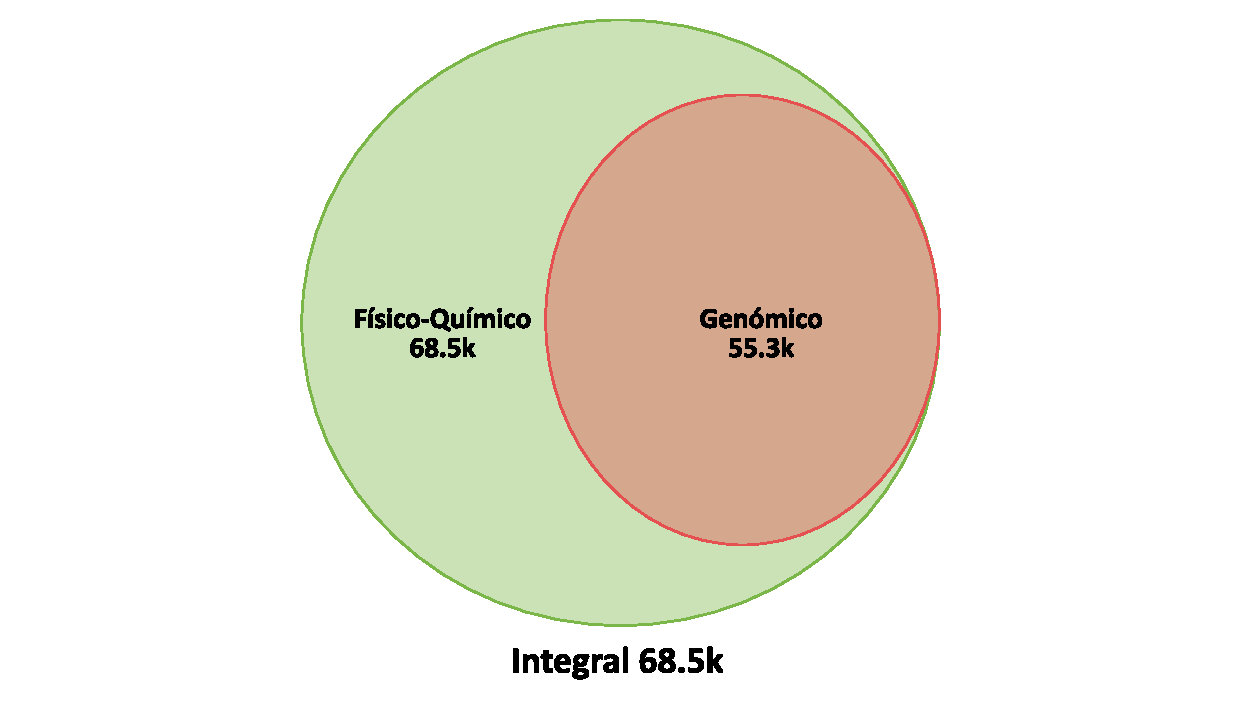
\includegraphics[width=2.60417in,height=\textheight]{interseccion_integral.pdf}
\caption{Unión de los datasets Físico-Químico y Genómico}
\end{figure}

\end{frame}

\begin{frame}{XGBoost supera a Random Forest}
\protect\hypertarget{xgboost-supera-a-random-forest}{}

\begin{columns}[T]
\begin{column}{0.48\textwidth}
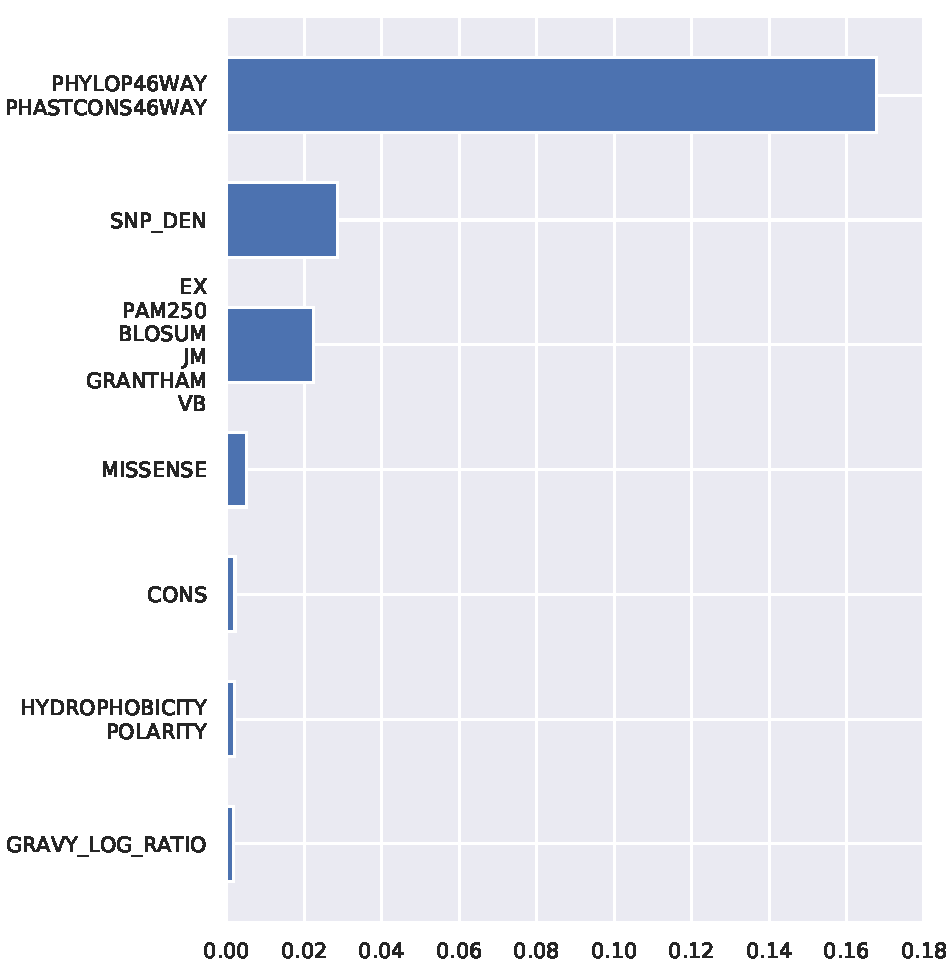
\includegraphics[width=2.44792in,height=\textheight]{integral_importance_cluster_xgb.pdf}
\end{column}

\begin{column}{0.48\textwidth}
\begin{figure}
\centering
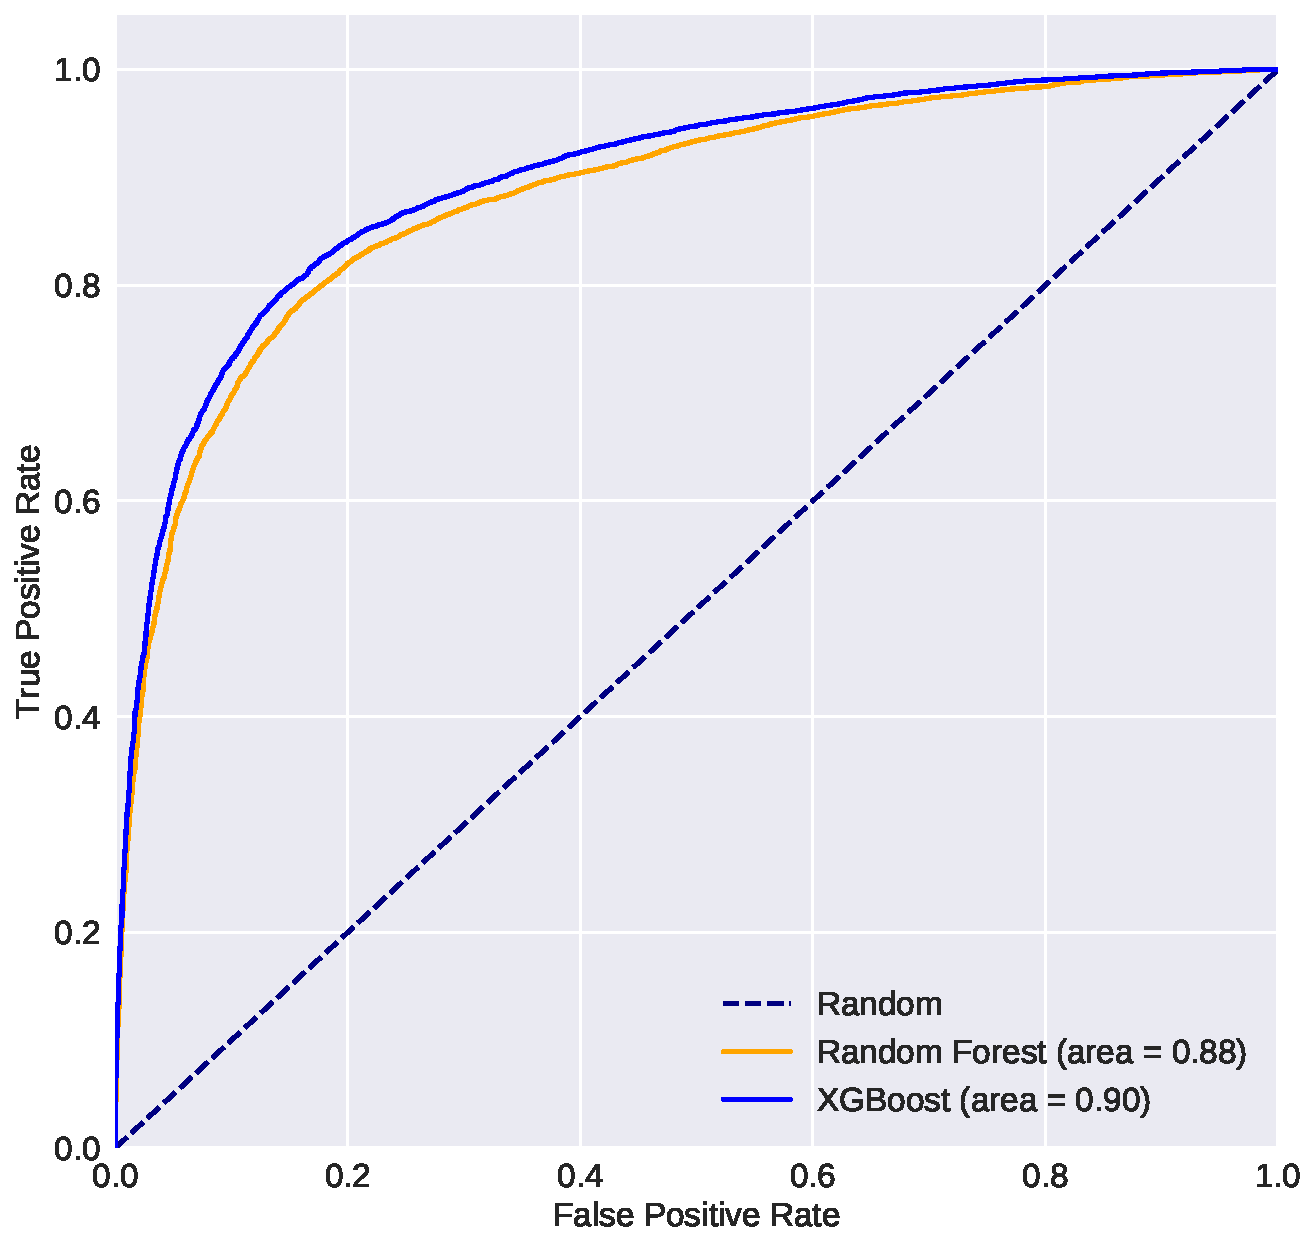
\includegraphics[width=2.08333in,height=\textheight]{auc_integral.pdf}
\caption{AUC: 0.90}
\end{figure}
\end{column}
\end{columns}

\end{frame}

\begin{frame}{Modelo Integral + VarQ}
\protect\hypertarget{modelo-integral-varq}{}

\begin{figure}
\centering
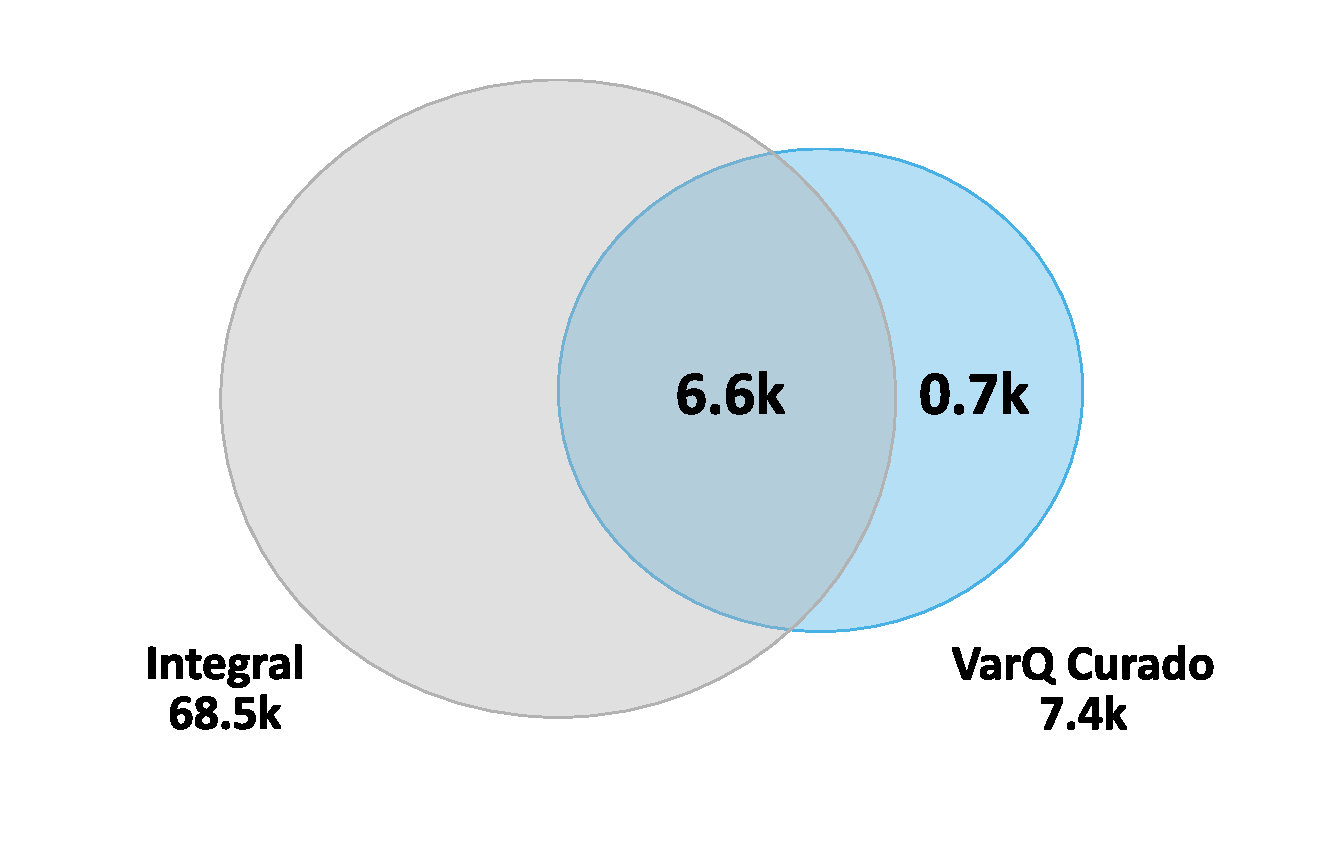
\includegraphics[width=3.125in,height=\textheight]{interseccion_varq_integral.pdf}
\caption{Unión de los datasets Integral y VarQ}
\end{figure}

\end{frame}

\begin{frame}{Resultados del modelo Integral + VarQ (XGBoost)}
\protect\hypertarget{resultados-del-modelo-integral-varq-xgboost}{}

\begin{columns}[T]
\begin{column}{0.48\textwidth}
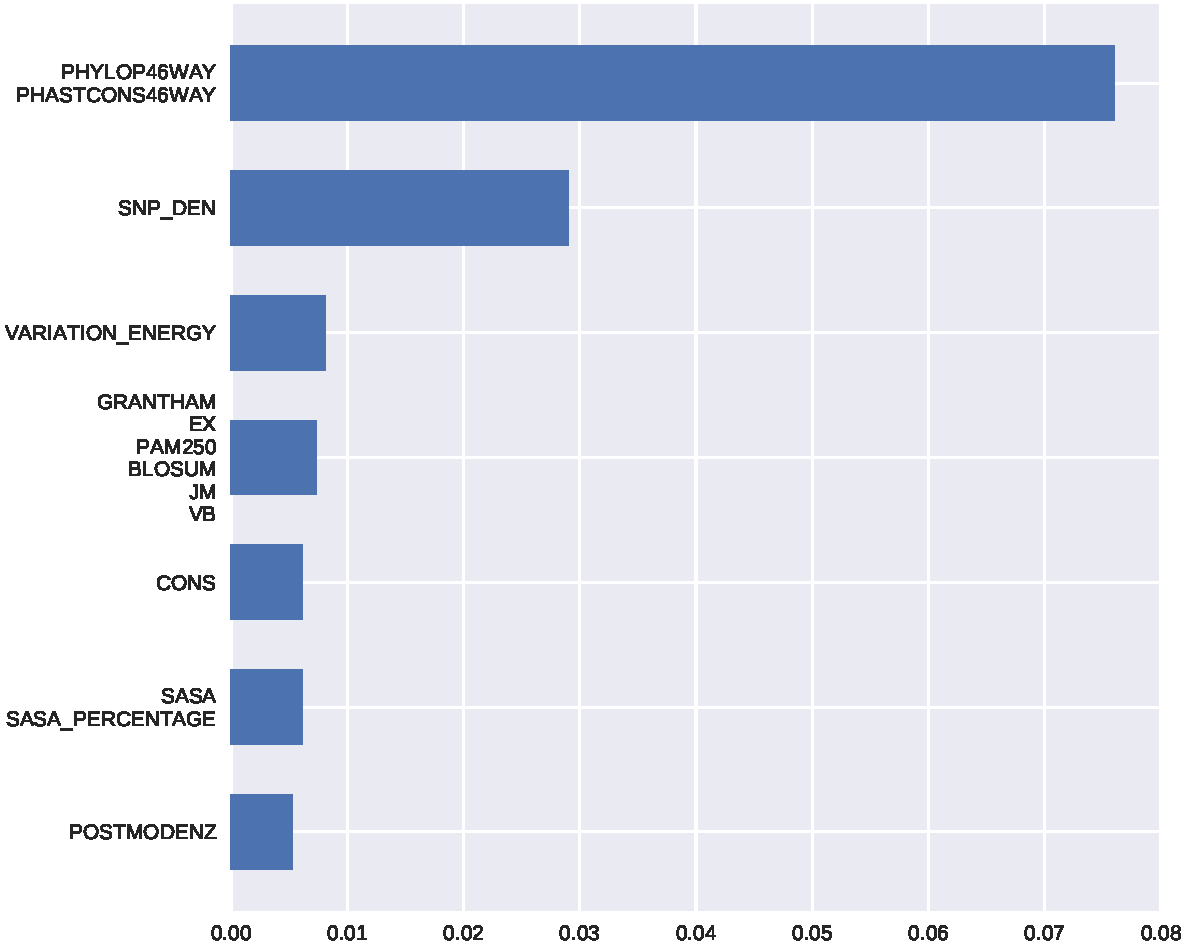
\includegraphics[width=2.44792in,height=\textheight]{integral_varq_importance_cluster_xgb.pdf}
\end{column}

\begin{column}{0.48\textwidth}
\begin{figure}
\centering
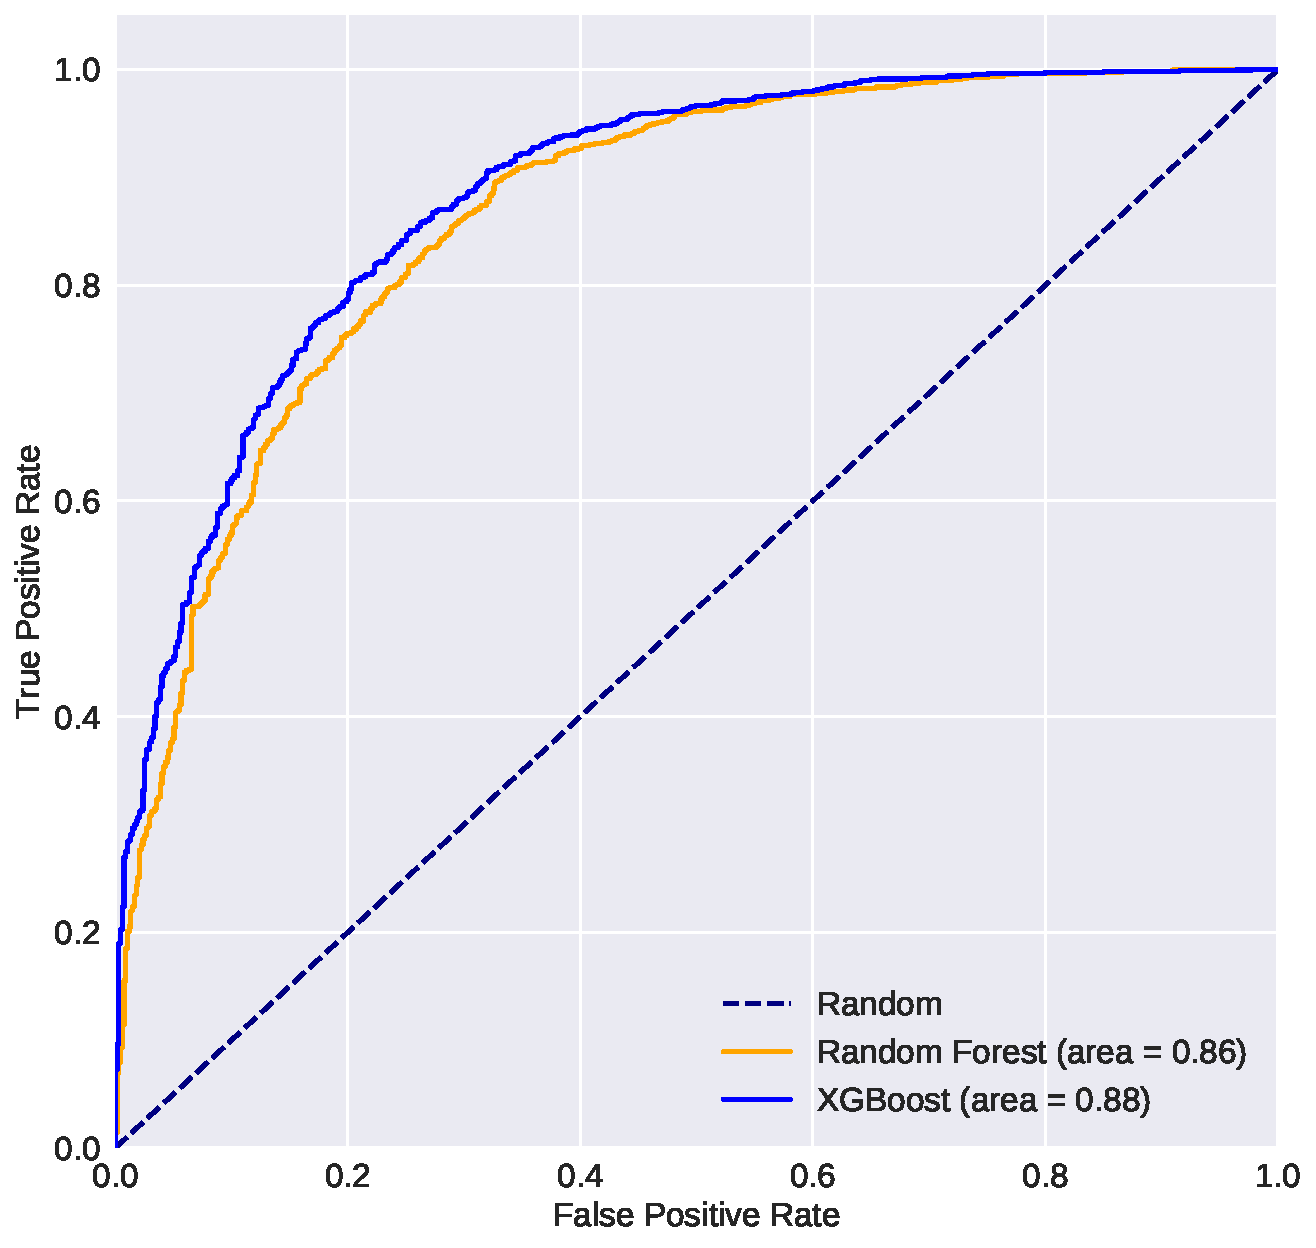
\includegraphics[width=1.82292in,height=\textheight]{auc_varq_integral.pdf}
\caption{AUC: 0.88}
\end{figure}
\end{column}
\end{columns}

\end{frame}

\begin{frame}{Comparación entre los distintos modelos}
\protect\hypertarget{comparaciuxf3n-entre-los-distintos-modelos}{}

\begin{columns}[T]
\begin{column}{0.48\textwidth}
\begin{figure}
\centering
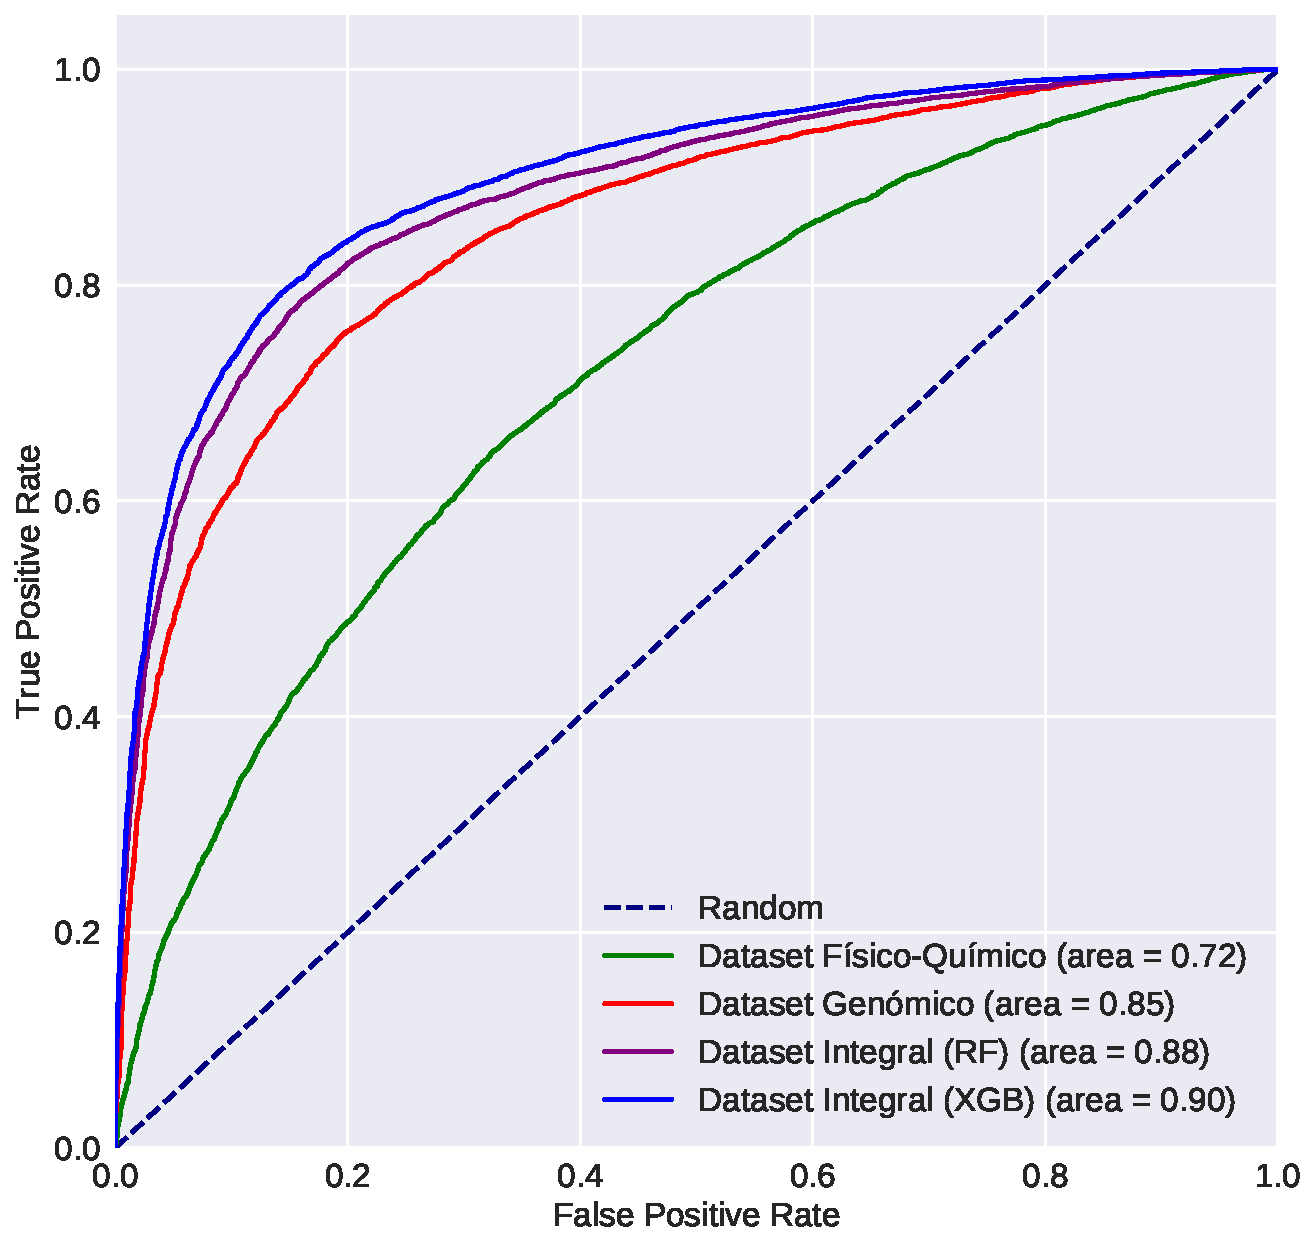
\includegraphics[width=2.08333in,height=\textheight]{curvas_auc_humsavar.pdf}
\caption{Dataset Humsavar}
\end{figure}
\end{column}

\begin{column}{0.48\textwidth}
\begin{figure}
\centering
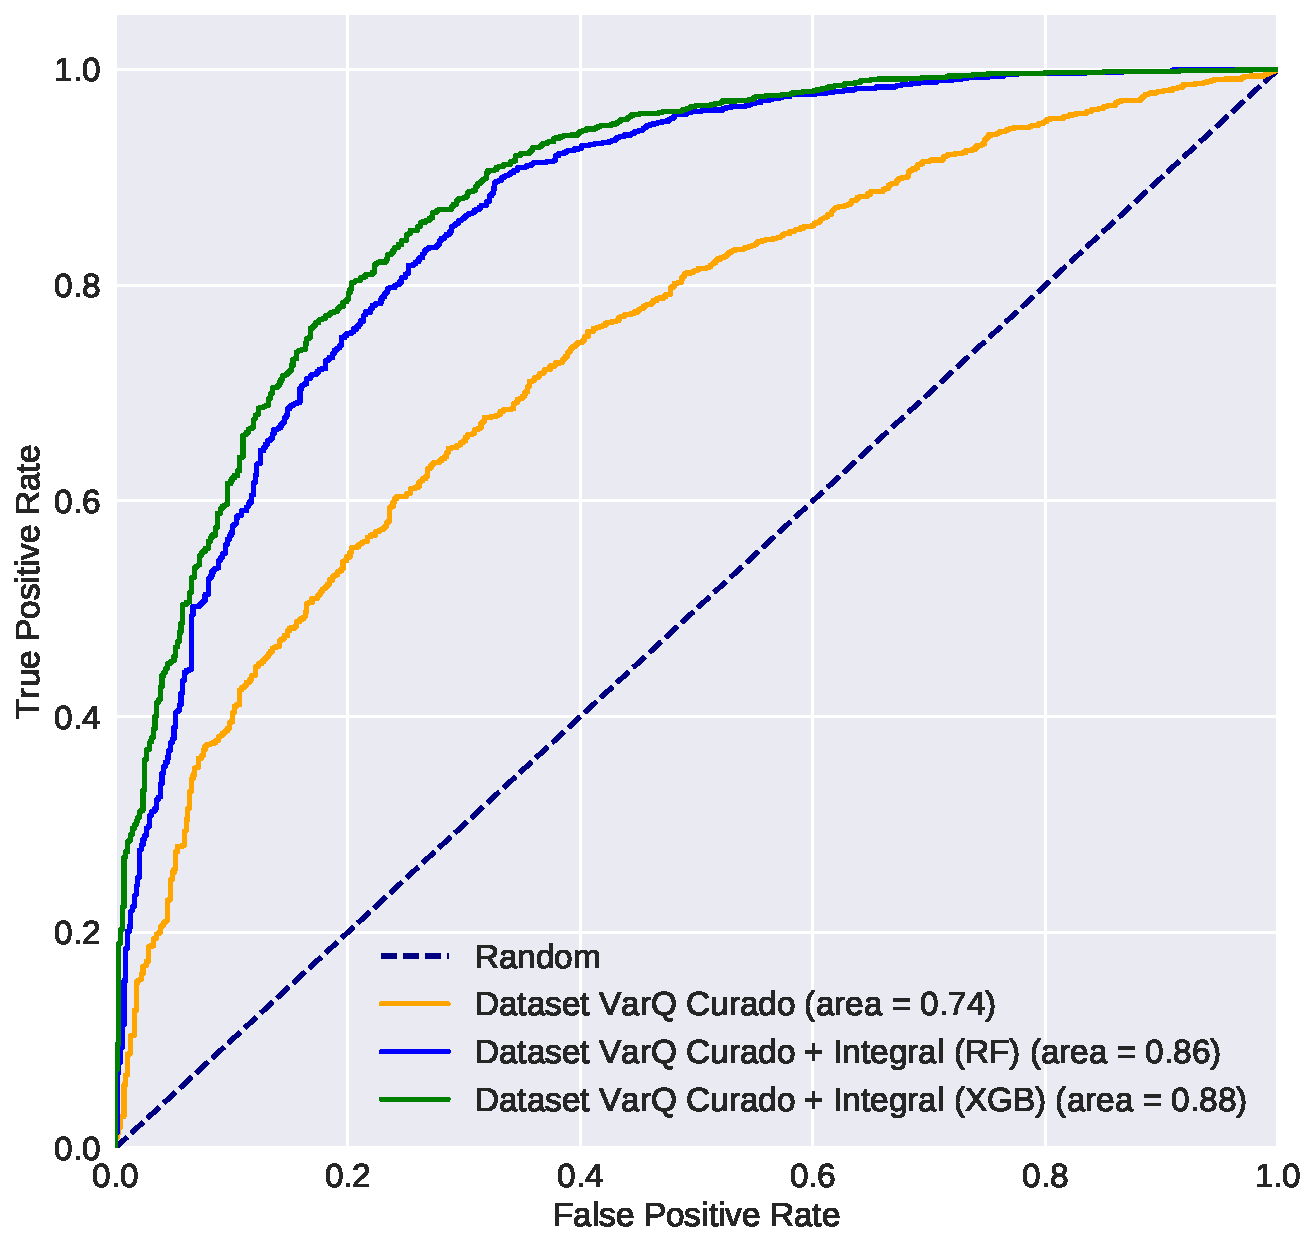
\includegraphics[width=2.08333in,height=\textheight]{curvas_auc_varq.pdf}
\caption{Dataset VarQ (Curado)}
\end{figure}
\end{column}
\end{columns}

\end{frame}

\begin{frame}{Conclusiones:}
\protect\hypertarget{conclusiones}{}

\begin{itemize}
\tightlist
\item
  La combinación de distintas dimensiones del problema aportó buenos
  resultados, consiguiendo un AUC de 0.90
\item
  El método estándar de cálculo de importancia de variables usado por
  scikit-learn puede ser engañoso en el caso de variables altamente
  correlacionadas
\item
  Los mejores resultados fueron obtenidos por algoritmos de Boosting
\end{itemize}

\end{frame}

\begin{frame}{Trabajo futuro}
\protect\hypertarget{trabajo-futuro}{}

\begin{itemize}
\tightlist
\item
  Aumentar la cobertura de las variables más importantes: La variación
  de la energía y las variables de conservación genómica
\item
  Mejorar la búsqueda de hiperparámetros en XGBoost
\item
  Evaluar SNPs \textit{nonsense} o no codificantes
\item
  Mejoras metodológicas
\end{itemize}

\end{frame}

\begin{frame}{}
\protect\hypertarget{section-4}{}

\begin{center}
\Huge ¿Preguntas?
\end{center}

\end{frame}

\begin{frame}{}
\protect\hypertarget{section-5}{}

\begin{center}
\Huge ¡Muchas gracias!
\end{center}

\end{frame}

\end{document}
